Una vez definido el diseño general del sistema, en este capítulo se detallan los agentes especializados que acceden a las fuentes de datos del proyecto software.

Para ello, se introduce primero la estructura de la clase base \opus{SpecializedAgent}, para posteriormente detallar las herramientas y la lógica de ejecución de los cinco agentes especialistas que extienden esta base.

\section{Estructura SpecializedAgent}
El grafo común de este agente comprende tres pasos principales: la configuración del prompt inicial mediante la función \opus{prepare_prompt()}, heredada de \opus{BaseAgent} y posteriormente extendida por cada agente especialista, la ejecución de un subgrafo que implementa el patrón ReAct (véase la Sección \ref{sec:react}) y la ejecución de un agente resumidor cuando sea necesario. La Figura \ref{fig:specialized} ilustra dicho flujo de ejecución.

\begin{figure}[h]
  \centering
  \adjustbox{center=\textwidth}{\hspace{-1.2cm}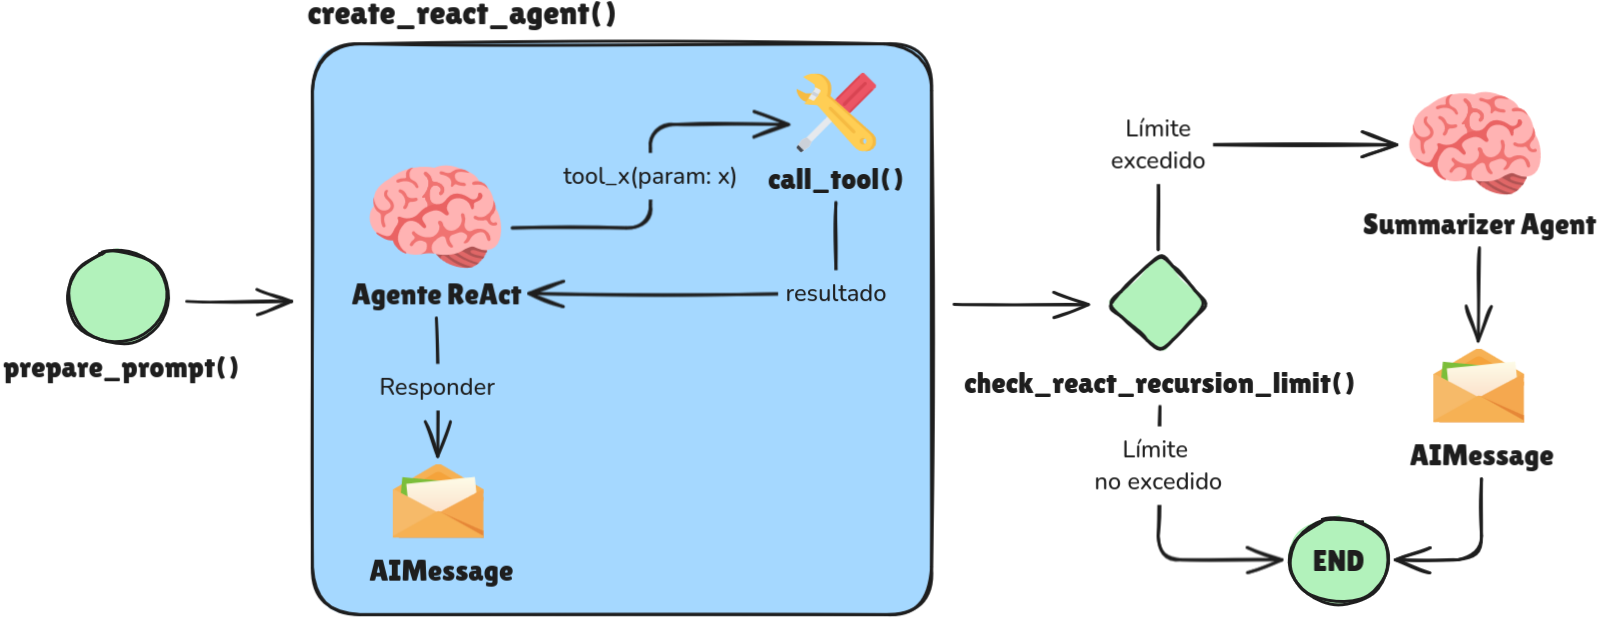
\includegraphics[width=1.2\linewidth]{figures/specialized.png}}
  \caption{Grafo de ejecución de agentes especializados}
  \label{fig:specialized}
\end{figure}

El grafo ReAct se ha implementado utilizando el agente prefabricado \opus{create_react_agent()} de LangGraph. Este agente acepta una serie de herramientas y un prompt inicial, entrando en un bucle de ejecución donde el agente invoca herramientas y observa sus resultados. El grafo finaliza cuando el mensaje del agente no contiene llamadas a herramientas, es decir, cuando incluye la respuesta final.

Se ha establecido un límite de iteraciones para el grafo ReAct, ya que se ha observado que ocasionalmente entra en un bucle excesivamente extenso al no encontrar la información requerida. Cuando se alcanza dicho límite, un agente resumidor genera una respuesta con la información disponible, observando todas las ejecuciones de las herramientas. 

El Listado \ref{lst:spec_graph} ilustra la creación del grafo para los agentes especialistas, añadiendo un nodo para cada etapa mencionada. El condicional \opus{check_react_recursion_limit} dirige la ejecución al nodo resumidor en caso de haber sobrepasado el límite de pasos en el agente ReAct.

\begin{lstlisting}[caption={\protect\opus{create_graph}: grafo de agentes especializados},label={lst:spec_graph}]
  def create_graph(self) -> CompiledGraph:
      # Crear grafo ReAct
      agent_tools = self.get_agent_tools()
      self.react_graph = create_react_agent(
          model=self.model,
          tools=agent_tools,
          checkpointer=self.checkpointer
      )

      # Crear grafo del SpecializedAgent
      graph_builder = StateGraph(AgentState)

      # Añadir nodos 
      graph_builder.add_node("prepare", self.prepare_prompt)
      graph_builder.add_node("react", self.call_langgraph_react_graph)
      graph_builder.add_node("response_summarizer", self.generate_summarized_response)

      # Establecer flujo entre nodos 
      graph_builder.set_entry_point("prepare")
      graph_builder.add_edge("prepare", "react")
      graph_builder.add_conditional_edges("react", self.check_react_recursion_limit)

      return graph_builder.compile()
\end{lstlisting}

Para acceder al estado de ejecución del agente ReAct tras finalizar abruptamente por el límite de mensajes, se utiliza el sistema de autoguardado de LangGraph. En la inicialización del agente se crea un objeto \opus{AsyncPostgresSaver}, vinculado a la base de datos PostgreSQL mediante un pool de conexión asíncrono y al contexto de cierre asíncrono \opus{global_exit_stack}. De este modo, todos los estados de ejecución se almacenan en una colección de PostgreSQL y son accesibles mediante su identificador. El autoguardado asíncrono previene problemas de concurrencia al ejecutar múltiples agentes asíncronos.

\subsection{Gestión de herramientas}
Algunas herramientas proporcionadas por los servidores MCP resultan innecesarias o contraproducentes para determinados agentes. Para evitar incluir contenido innecesario en los prompts, se debe indicar al instanciar un agente el nombre de las herramientas que se utilizarán, filtrando posteriormente las herramientas en el cliente.

Por otra parte, algunos servidores MCP no proporcionan todas las funcionalidades requeridas. Para obtener estas herramientas adicionales, la función \opus{add_additional_tools()} incorpora, cuando es necesario, herramientas complementarias específicas para cada agente.

\subsection{Sistema de citas}
Para que el usuario final obtenga las fuentes de información utilizadas en la respuesta a su consulta, los agentes especializados deben referenciar los documentos consultados. Un sistema sencillo podría solicitar en el prompt que el agente indique la ruta o nombre del archivo, pero sería propenso a errores debido a que las direcciones URL de cada fuente de datos siguen patrones diferenciados. Para garantizar que los documentos citados siempre existan y contengan una dirección válida, se ha implementado el sistema ilustrado en la Figura \ref{fig:citations}.

\begin{figure}[h]
  \centering
  \adjustbox{center=\textwidth}{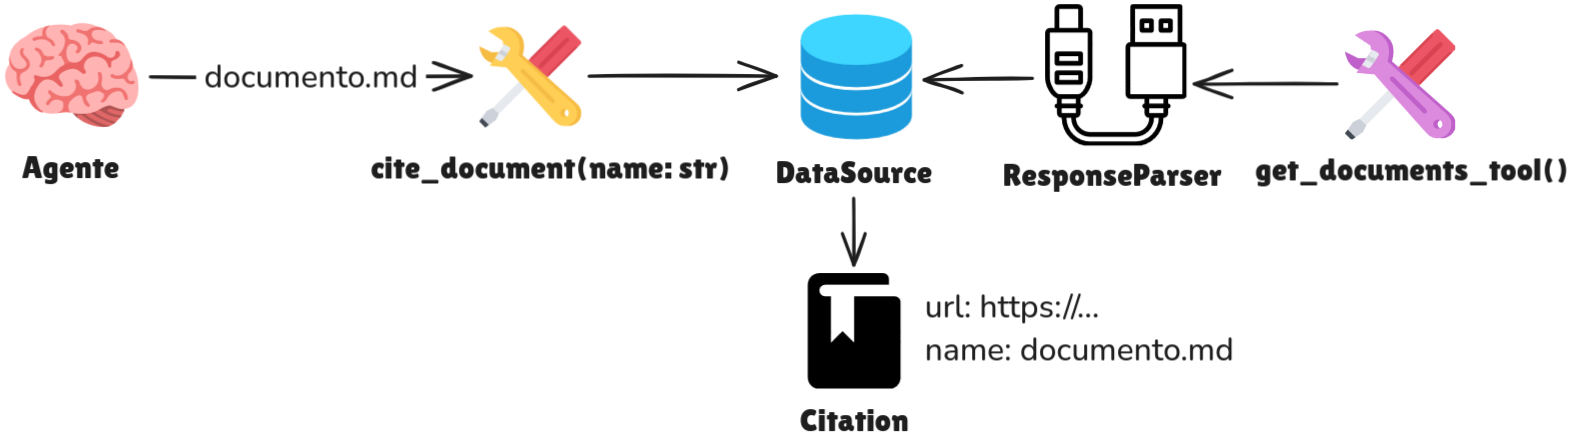
\includegraphics[width=1.1\linewidth]{figures/citations.png}}
  \caption{Diagrama de funcionamiento del sistema de citas}
  \label{fig:citations}
\end{figure}
Este diseño proporciona a cada agente una herramienta para citar documentos de las fuentes de datos disponibles. La herramienta se construye dinámicamente para cada agente según las fuentes de datos a las que tiene acceso. Para ello, se implementa la clase \opus{DataSource} ilustrada en el Listado \ref{lst:data_src}, la cual se instancia en la conexión al servidor MCP y almacena todos los documentos citables.

Esta clase almacena un identificador único para la fuente de datos, la URL común a todos los documentos y un diccionario con el nombre de cada documento asociado a su URL complementaria. Asimismo, cada fuente de datos se asocia a un \opus{ResponseParser}, que convierte el nombre del documento en el enlace completo considerando el prefijo común de la fuente y el prefijo del documento. Por ejemplo, en Confluence, la URL de un documento sigue la estructura \opus{url_confluence/tipo_documento/id_documento/nombre_documento}, por lo que su parser construye la URL añadiendo el prefijo correspondiente al tipo de documento y su ID.

\begin{lstlisting}[caption={\protect\opus{DataSource}: clase destinada a almacenar los documentos citables para una fuente de datos}, label={lst:data_src}]
class DataSource(ABC):
    url: str
    # Nombre de herramienta para obtener la lista de documentos disponibles
    get_documents_tool_name: str | List[str]
    # Nombre del documento junto al prefijo necesario en la url
    available_documents: dict[str, str]
    # Identificador de la fuente de datos
    docs_id: str
    parser: ResponseParser
\end{lstlisting}

Por lo tanto, el agente dispondrá de una herramienta donde bastará con indicar el nombre del documento a citar. El agente podrá citar la propia fuente de datos utilizando el nombre especificado en la descripción de la herramienta. Las citas se propagarán mediante objetos estructurados por toda la arquitectura de agentes para imprimir finalmente las citas empleadas, como se explica en la Sección \colorbox{yellow}{\ref{}}.


\section{Agentes implementados}
En esta sección se detallan los cinco agentes desarrollados que extienden las funcionalidades descritas en la sección anterior.

\subsection{Agente código}
El flujo de este agente comprende el siguiente proceso: mediante \opus{prepare_prompt()} se incluye en el prompt del sistema el árbol de directorios del repositorio obtenido con la herramienta \opus{get_repository_tree_tool} y fragmentos de código, denominados \textit{chunks}, relevantes para la consulta actual obtenidos mediante la herramienta \opus{get_code_repository_rag_docs_from_query_tool}. Tras concatenar la consulta al agente mediante un \opus{HumanMessage}, este debe decidir si buscar chunks adicionales sobre un subdirectorio concreto indicando otra consulta, buscar archivos específicos con la herramienta \opus{get_file_from_repository_tool} indicando su ruta relativa, o responder directamente a la consulta.

Los chunks devueltos por dicha herramienta contienen tanto el código como la ruta relativa del archivo donde se declaran, permitiendo buscar en dicho archivo si fuese necesario. Adicionalmente, al extraer un chunk, se incluyen chunks referenciados o que referencian ese fragmento. Se define que un chunk referencia a otro cuando llama a una función o instancia una clase definida en el otro chunk. La cantidad de chunks referenciados y que referencian se limita a uno por chunk, y la cantidad total de chunks por cada llamada a la herramienta se limita a tres. Esta reducción en el número de chunks favorece múltiples llamadas con consultas variadas.

\subsubsection{Herramientas de acceso a código}
Para implementar las herramientas de este agente, en el componente \opus{servidor_mc_bd_codigo} se han dividido los ficheros del proyecto GitLab en \textit{chunks} y posteriormente se han indexado en la base de datos Postgres.

Para implementar este sistema RAG, se ha utilizado la extensión PGVector sobre PostgreSQL. Dicha extensión ofrece la opción de mezclar vectores embeddings en una tabla SQL tradicional, proporcionando operaciones de búsqueda semántica combinadas con operaciones SQL. Para ello, se ha definido el modelo relacional ilustrado en la Figura \ref{fig:relacional}, implementando el modelo ORM de SQLAlchemy sobre Python. El diseño se basa en una tabla \opus{FileSystem} para cada fichero o directorio, la cual puede contener varios \opus{FileChunk} indexados en la columna \opus{embedding} de tipo \opus{Vector}. Además, cada \textit{chunk} puede referenciar o ser referenciado por otros \textit{chunk}, en caso de que el chunk referenciado contenga una clase o función definida en el chunk referenciador. La tabla \opus{Ancestor} constituye un patrón de tabla de cierre para acceder eficientemente a todos los ficheros dentro de un subdirectorio. 

\begin{figure}[h]
  \centering
  \adjustbox{center=\textwidth}{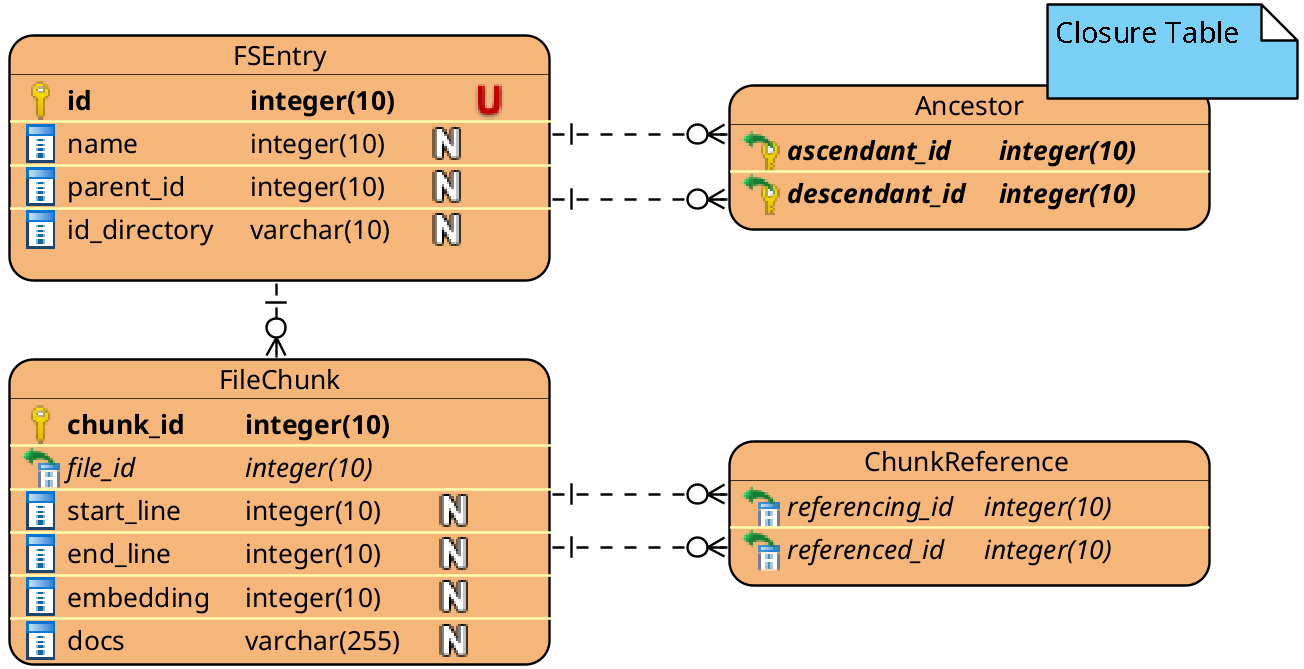
\includegraphics[width=0.95\linewidth]{figures/db.png}}
  \caption{Diagrama relacional de la base de datos con el código fuente del proyecto software}
  \label{fig:relacional}
\end{figure}

\paragraph{Procedimiento de chunking}
Para realizar la división de los ficheros en \textit{chunks}, se han considerado las clases y funciones que componen el código. Un agente se beneficiará mucho más si el segmento de código al que tiene acceso no contiene definiciones de clases o funciones a medias. Para ello, se ha utilizado la librería grep-ast\footnote{grep-ast: \url{https://github.com/Aider-AI/grep-ast}}. Esta librería recibe ficheros de un lenguaje de programación concreto, e identifica las definiciones (declaraciones de funciones y clases), y las referencias (cuando en un segmento de código se llama a una clase o función, entonces este segmento contiene una referencia a otro segmento). 

Una vez obtenidas todas las definiciones declaradas en un fichero, se debe dividir el fichero en bloques de tamaño parecido. Para intentar no dividir definiciones de funciones o clases en diferentes chunks, se ha utilizado el patrón State ilustrado en la Figura \ref{fig:chunks}. Este comienza por el principio del fichero y empieza a añadir definiciones secuencialmente al chunk actual. En caso de que la siguiente definición no quepa en el chunk actual y el chunk actual contenga alguna definición, se crea el chunk actual (añadiendolo a la base de datos) y se vacía el chunk actual en el agloritmo. En caso de que el chunk actual esté vacío, significa que el siguiente chunk es demasiado grande para entrar en un solo chunk, por lo que es necesario dividirlo. Para ello, en caso de que sea una función se divide y se crean los chunks con un tamaño igual. en caso de qeu sea una clase, se pasa a un proceso similar pero con las funciones dentro de la misma clase, para intentar no dividr las funciones dentro de la definición de la clase. Una vez se han añadido todas las definiciones, en caso de existir líneas al final del fichero no pertenecientes a ninguna definición, se intentan añadir a la última definición.

\begin{figure}[h]
  \centering
  \adjustbox{center=\textwidth}{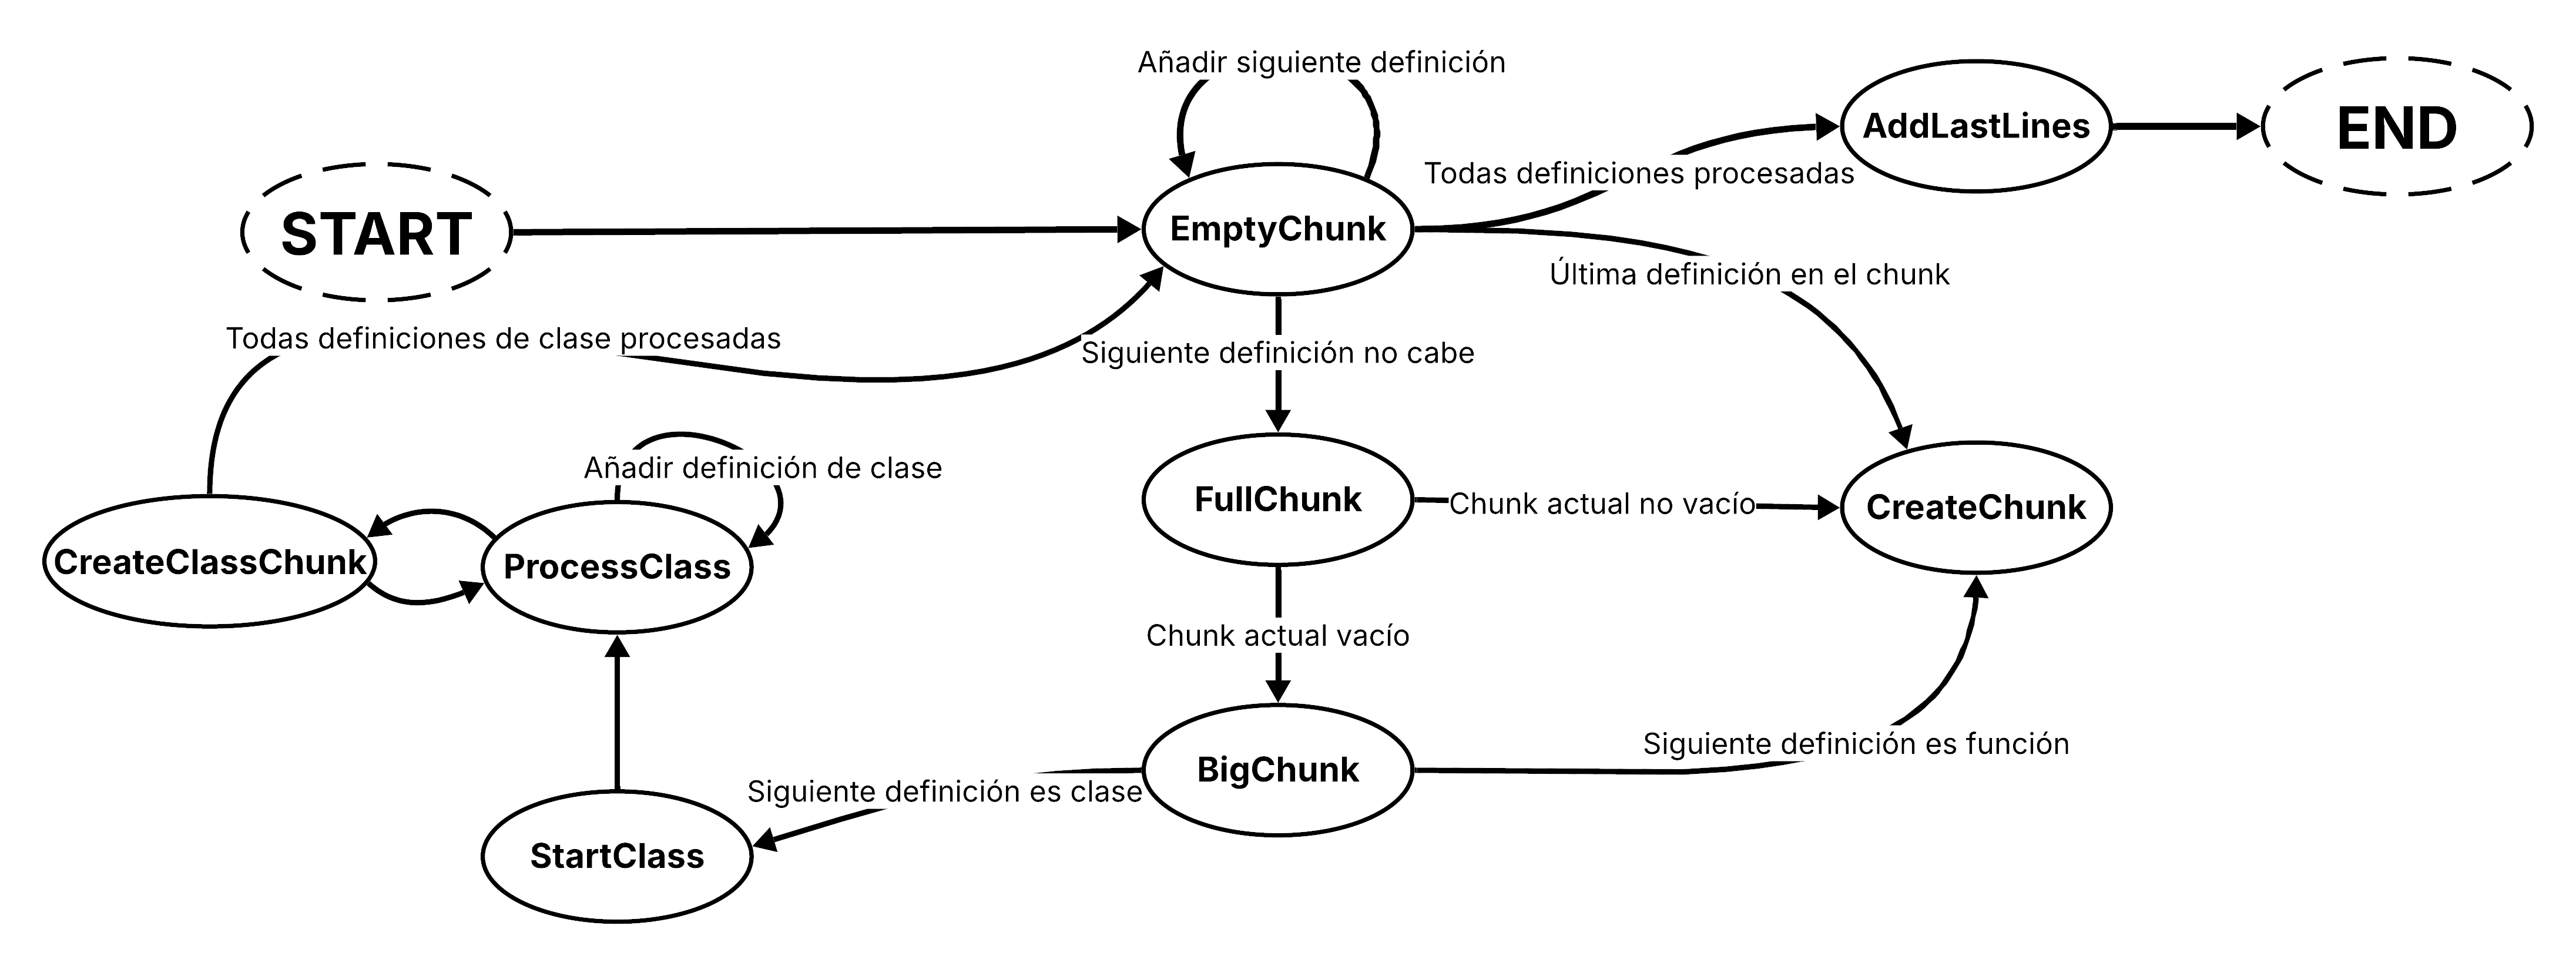
\includegraphics[width=1.35\linewidth]{figures/chunks.png}}
  \caption{Algoritmo de chunking considerando definiciones de funciones y clases en el código fuente}
  \label{fig:chunks}
\end{figure}

Consecuentemente, el proceso de chunking sigue el siguiente procedimiento: una función recursiva obtiene los directorios y ficheros a ignorar para el proceso de chunking y comienza el proceso desde el directorio raíz. Se listan los elementos dentro del directorio actual y se procesan uno a uno. En caso de encontrar un directorio, se llama a la función de forma recursiva para este directorio. En caso de ser un fichero, se obtienen las definiciones y referencias dentro del fichero mediante la librería mencionada. Con el patrón State mencionado se dividen los ficheros con dichas definiciones en chunks. Tras dividir cada chunk, se van anotando en un diccionario el nombre de las definiciones declaradas junto al identificador del chunk en el que se declaran. Lo mismo se hace para el nombre de las referencias junto al identificador de los chunks donde se declaran. Una vez finalizado el procesado de los chunks, un algoritmo asigna las referencias declaradas a las definiciones declaradas, creando las relaciones de referencia en el modelo de la Figura \ref{fig:relacional}.

Para verificar el correcto funcionamiento de este procedimiento, se han creado nueve tests unitarios de caja negra para las funcionalidades principales del chunking con la librería pytest\footnote{pytest: \url{https://docs.pytest.org/en/stable/}}. Estos tests se enfocan en la correcta identificación de definiciones y clases, así como la correcta división de los chunks para los casos más infrecuentes. Estos tests se han configurado de forma que se ejecuten automáticamente en cada push a las ramas develpo o master, mediante un pipeline integrado a SonarCloud\footnote{SonarCloud: \url{https://www.sonarsource.com/products/sonarcloud/}}, para mostrar la covertura de código en dicha plataforma.  

\paragraph{Procedimiento de indexación}
Para indexar cada chunk, en lugar de indexar directamente el código fuente, se ha indexado de forma que cada chunk una plantilla conteniendo el chunk a indexar, todo el fichero del que el chunk es parte, el árbol completo del repositorio y la documentación API generada por el agente RepoAgent.  

Esta indexación requiere de varias operaciones a nivel de repositorio, fichero y chunks. Además, devido al coste computacional de la indexación, es necesario procesarlo de forma asíncrona. Para ello, se ha creado un algoritmo de indexación siguiendo el patrón Pipeline\footnote{Patrón Pipeline: \url{https://medium.com/@bonnotguillaume/software-architecture-the-pipeline-design-pattern-from-zero-to-hero-b5c43d8a4e60}}. Este patrón desacopla el proceso de iteración de las operaciones a realizar, añadiendo diferentes procesos a realizar en dos stages de la indexación, cada uno con un dataclass con atributos requeridos en dicha operación:
\begin{itemize}
  \item\textbf{PipelinePipelineStage: }Procesos a ejecutar para todo el repositorio al inicio del procedimiento. Se consideran la creación del árbol de directorios del repositorio mediante la librería treelib\footnote{treelib: \url{https://pypi.org/project/treelib/}}, la creación de la documentación API mediante el agente RepoAgent, cuya ejecución se ilustra en el Listado \ref{} 
  \item\textbf{FilePipelineStage: }Procesos a ejecutar para cada fichero. En esta implementación no ha sido necesario ningún proceso a este nivel, se define para que guardar el estado y la ejecución de cada fichero de forma estructurada. 
  \item\textbf{ChunkPipelineStage: }Procesos a ejecutar para cada chunk. Aquí se consideran la creación de la documentación a utilizar y la indexación de dicha documentación. 
\end{itemize}

De esta forma, al ejecutar el pipeline completo, primero se ejectuan las operaciones a nivel de repositorio, después se ejecutarán las operaciones a nivel de fichero de forma asíncrona, permitiendo el log del procesado de cada fichero de forma estructurada, y finalmente se ejecutarán las operaciones a nivel de chunk de forma asíncrona. Las operaciones dentro de cada nivel de ejecución se ejecutarán secuencialemente, es decir, para cada chunk, primero se ejecutará el proceso de generar la documentación y posteriormente la de indexar dicha documentación. 


\begin{lstlisting}[caption={\protect\opus{generate_extra_docs}: Ejecución de agente RepoAgent para crear la documentación API}, label={lst:spec_graph}]
  def generate_extra_docs(files_to_ignore: List[str], repo_path: str, extra_docs_path: str):
      try:
          files_to_ignore_str = ",".join(files_to_ignore)
          command = f"repoagent run --model gpt-4o-mini --target-repo-path {repo_path} --markdown-docs-path {extra_docs_path} --ignore-list {files_to_ignore_str}"
          exit_code = execute_and_stream_command(command)
      ...
\end{lstlisting}

\subsection{Agente Google Drive}
La función de este agente es buscar y analizar las maquetas HTML disponibles en Google Drive. Para ello, mediante la heramienta \opus{gdrive_list_files()}, la función \opus{prepare_prompt()} le indica todos los documentos disponibles. Posteriormente, este tiene que decidir si buscar fragmentos relevantes en los documentos mediante la herramienta de búsqueda \opus{gdrive_search()}, o leer documentos enteros mediante la herramienta \opus{gdrive_read_file()}.

\subsection{Agente Sistema de Ficheros}
Este debe responder a consultas de diversas temáticas utilizando la fuente de datos de la documentación oficial. Para ello, similar al agente anterior, recibe la lista de documentos disponibles con la herramienta \opus{directory_tree()}, y puede decidir cuáles documentos necesita leer con las herramientas \opus{read_file()} o \opus{read_multiple_files()}. En caso de no saber exactamente cuál documento leer, puede buscar pasajes relevantes mediante la herramienta \opus{rag_search_documentation()}, la cual devuelve dichos fragmentos y el nombre del documento en los que se declaran.

Esta última herramienta se implementado mediante la clase \opus{PGVector} de LangChain. A diferencia de la implementación para el agente de código, esta es una abstracción sobre el plugin de PGVector. Ofrece la capacidad búsquedas RAG de forma sencilla, pero sin la opción de combinar operaciones de búsqueda semántica con búsquedas SQL. Como se muestra en el Listado \ref{lst:pgvector_store}, se crean colecciones instanciando la clase PGVector, y posteriormente se pueden añadir o buscar documentos relevantes con sus respectivas funciones. La clase espera un diccionario de elementos, de los cuales una columna se indexará (se convertirá en un vector numérico para realizar la búsqueda), y las demás servirán de metadatos. Es posible filtrar en las búsquedas por metadatos, pero se pierde la capacidad de PGVector nativo para realizar consultas en diferentes tablas. 

\begin{lstlisting}[caption={\protect\opus{PGVector}: uso de clase para indexar o buscar documentos}, label={lst:pgvector_store}]
  # Instanciar la clase en su versión asíncrona 
  vector_store = PGVector(
      embeddings=self.embeddings,
      collection_name=prefixed_name,
      connection=self.engine,
      use_jsonb=True,
      async_mode=True
  )

  # Añadir documentos (clase LangChain con texto y metadatos) al store
  await self.vector_store.aadd_documents(docs)

  # Buscar documentos similares mediante una operación vectorial
  results = await self.vector_store.asimilarity_search(query, k=top_k)
\end{lstlisting}

\subsection{Agente Confluence}
Para este agente se han implementado dos versiones alternativas, una similar a los anteriores y otra con cacheo de prompt de todos los documentos, para poder comparar y sacar conclusiones en la fase de evaluación.

El \textit{prompt caching} consiste en guardar la representación interna de los LLM para una secuencia de texto concreta inicial para no tener que repetir los cálculos necesarios si en una consulta posterior se repite ese fragmento inicial. De esta forma, las API como openai ofrecen descuentos significativos si se cachea gran parte de la entrada.

\paragraph{Sin prompt caching}
Similar a los agentes anteriores, con la herramienta \opus{confluence_search()} se le indican los documentos disponibles en la documentación del estilo visual del proyecto, y con \opus{confluence_get_page()} debe decidir cuáles documentos leer. 

\paragraph{Con prompt caching}
En esta versión el agente recibe directamente toda la documentación en su contexto de entrada, y debe responder directamente citando los documentos necesarios. Es de destacar que esta estrategia funciona únicamente en los casos en los que los documentos caben en la ventana de contexto del modelo.

\subsection{Agente GitLab}
Para este agente se han tenido que implementar una serie de herramientas utilizando directamente la API de GitLab como se explica en la Sección \ref{}. Para ello se ha utilizado la librería \opus{requests}.

Este agente recibe en el \opus{SystemMessage} estadísticas del repositorio con la herramienta \opus{get_gitlab_project_statistics()}, con información como la cantidad de contribuciones, usuarios o incidencias en el repositorio. Posteriormente, este puede llamar a las siguientes herramientas:
\begin{itemize}
  \item\opus{get_gitlab_project_commits(user_name, since, until, result_limit): } Obtener las contribuciones (\textit{commits}) al repositorio, opcionalmente filtrando por usuarios, fechas o cantidad de resultados.
  \item\opus{get_gitlab_project_members(): }Obtener información sobre los usuarios contribuyentes al proyecto. Es de destacar que si se quiere filtrar por contribuyentes en la herramienta anterior, el agente debe razonar para llamar esta heramienta inicialmente para obtener los nombres de usuarios.
  \item\opus{get_gitlab_braches(): }Obtener información sobre las ramas git del proyecto
  \item\opus{get_gitlab_issues(): }Obtener las incidencias del proyecto.
\end{itemize}



















